\begin{exercise}
      {ID-ec09c5c5590a099daaa9d9e0ae2b1eb3136b2453}
      {Wasserstand}
  \ifproblem\problem\par
    % <PROBLEM>
    Der Wasserstand eines Flusses wird
    kontinuierlich an Pegellatten abgelesen
    und in Zentimetern über Pegelnull
    (cm ü PN) angegeben.
    \par
    Nach einer längeren Trockenperiode,
    in welcher der Wasserstand unter
    den Pegelnullpunkt gesunken ist,
    sorgten starke Regenfälle am
    Tage für einen Kurzfristigen
    Anstieg des Pegelstandes des Flusses.
    Über einen Zeitraum von 0 bis 24 Uhr
    soll der Pegelstand $f$ in Abhängigkeit
    von der Zeit $x$ ausgewertet werden.
    Der Pegelstand $f$ kann näherungsweise
    durch die Funktion $f$ mit
    \begin{equation*}
      f(x)=-\num{0.5}x^4+\num{3}x^2-\num{1}
      \quad,\quad
      x\in\mathbb{R}
      \quad,\quad
      0\leq x\leq\num{2.4}
    \end{equation*}
    dargestellt werden. Der Graph $G_f$ ist in der
    Skizze veranschaulicht. Eine Einheit auf der
    $y$-Achse entspricht \SI{10}{\centi\metre} und
    eine Einheit auf der $x$-Achse entspricht
    10 Stunden.
    \begin{center}
      %<OCTAVE>
      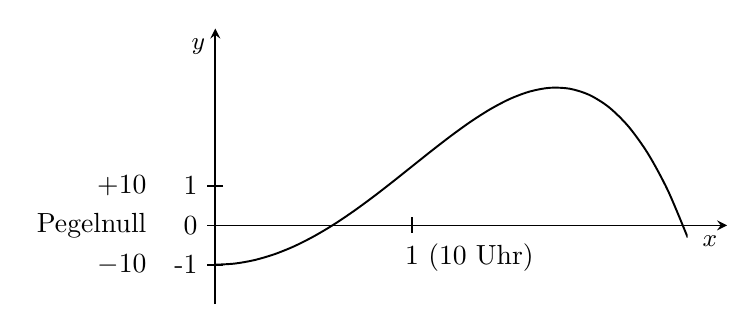
\begin{tikzpicture}[scale=0.500]
        % grid
        %\draw[draw=black!50!white] (0.000, -2.000) grid[step=0.5] (13.000, 5.000);
        % x-axis
        \draw[line width=0.6pt, ->, >=stealth] (0.000, 0) -- (13.000, 0) node[below left] {\small$x$};
        % y-axis
        \draw[line width=0.6pt, ->, >=stealth] (0, -2.000) -- (0, 5.000) node[below left] {\small$y$};
        \begin{scope}[xscale=5]
          % function: f(x)=-\num{0.5}x^{4}+\num{3}x^{2}-\num{1}
          \begin{scope}[line width=0.7pt]
            \clip (0.000, -2.000) rectangle (2.400, 5.000);
            \draw plot[smooth] coordinates
            {
              (  0.000,  -1.000) (  0.100,  -0.970) (  0.200,  -0.881)
              (  0.300,  -0.734) (  0.400,  -0.533) (  0.500,  -0.281)
              (  0.600,   0.015) (  0.700,   0.350) (  0.800,   0.715)
              (  0.900,   1.102) (  1.000,   1.500) (  1.100,   1.898)
              (  1.200,   2.283) (  1.300,   2.642) (  1.400,   2.959)
              (  1.500,   3.219) (  1.600,   3.403) (  1.700,   3.494)
              (  1.800,   3.471) (  1.900,   3.314) (  2.000,   3.000)
              (  2.100,   2.506) (  2.200,   1.807) (  2.300,   0.878)
              (  2.400,  -0.309)
            };
          \end{scope}
        \end{scope}
        % x labels
        \draw[line width=0.6pt] (5, 2mm) -- (5, -2mm) node[below]{1\makebox[0pt][l]{~(10 Uhr)}};
        % y labels
        \draw[line width=0.6pt] (2mm,  1) -- (-2mm,  1) node[left]{1};
        \draw[line width=0.6pt] (2mm,  0) -- (-2mm,  0) node[left]{0};
        \draw[line width=0.6pt] (2mm, -1) -- (-2mm, -1) node[left]{-1};
        \node[left] at (-1.5,  1) {$+\SI{10}{\centi\metre}$};
        \node[left] at (-1.5,  0) {Pegelnull};
        \node[left] at (-1.5, -1) {$-\SI{10}{\centi\metre}$};
      \end{tikzpicture}
      %</OCTAVE>
      %p = [-0.5 0 3 0 -1];
      %mypolyplot(p, 0, 2.4, -2, 5, 0.1, 0.5)
    \end{center}
    \begin{enumerate}[a)]
      %\setlength{\itemsep}{-1ex}%
      \item Weisen Sie rechnerisch nach, dass die Punkte
            $P_1\left(\num{0.7}\;\middle|\;\num{0.35}\right)$ und
            $P_2\left(\num{1.6}\;\middle|\;\num{3.40}\right)$
            zum Graphen der Funktion $f$ gehören, der die
            Pegelstände des Flusses zu bestimmten Zeiten
            beschreibt und geben Sie die dazugehörigen Uhrzeiten an.
            \par
            Berechnen Sie den Pegelstand zu Beginn der Messung
            und zeigen Sie rechnerisch, dass es sich um einen
            lokalen Tiefpunkt von $G_f$ handelt.
      \item Ermitteln Sie die Gesamtdauer der Zeit, in
            welcher der Pegelstand über dem Pegelnullpunkt lag.
      \item Geben Sie den Pegelstand um 20 Uhr an und ermitteln
            Sie rechnerisch in cm je Stunde, wie stark der
            Pegelstand zu diesem Zeitpunkt steigt bzw. fällt.
      \item Berechnen Sie den Zeitpunkt, an dem der Pegelstand
            am höchsten war und geben Sie den Pegelstand an.
      \item Bestimmen Sie die Koordinaten des Wendepunktes von
            $G_f$ und erläutern Sie die Bedeutung dieses
            Wendepunktes in Hinblick auf die Tendenz des
            Pegelstandes.
    \end{enumerate}
    % </PROBLEM>
  \fi
  %\ifoutline\outline\par
    % <OUTLINE>
    % </OUTLINE>
  %\fi
  %\ifoutcome\outcome\par
    % <OUTCOME>
    % </OUTCOME>
  %\fi
\end{exercise}
